\documentclass[hidelinks,a4paper]{article}

\usepackage[margin=1.5in]{geometry}
\usepackage[T1]{fontenc}
\usepackage{blindtext}
\usepackage{tgpagella}
\usepackage[activate=true,tracking=true,kerning=true,spacing=true,factor=2000,stretch=50,selected=true,letterspace=1000,final=true,verbose=true]{microtype}
\usepackage{fourier-orns}
\usepackage{titlesec}

\newcommand{\sectionbreak}{\clearpage}

\usepackage[english]{babel}
\usepackage[utf8]{inputenc}
\usepackage{amsmath}
\usepackage{graphicx}
\usepackage{wrapfig}
\usepackage[colorinlistoftodos]{todonotes}
\usepackage{hyperref}
\usepackage[toc,page]{appendix}

\title{getaLife}

\author{
  Minardi, Claudia\\
  \texttt{minardi.claudia@gmail.com}
  \and
  Ortega, Julian\\
  \texttt{jortegac@gmail.com}
  \and
  Stablum, Francesco\\
  \texttt{stablum@gmail.com}
}

\date{\today}

\begin{document}
\maketitle

\tableofcontents

\section{Introduction}

Looking for events online has become a common practice in order to get information
on how to spend ones free time. For this reason there has been a proliferation
of websites and underlying databases that aim to gather event data.
What they typically offer is a search form and then a tabular view of
the matching events.

What we offer is an innovative interface for performing similar queries.
In our system, the geographical map is center stage and gets populated by
the events that match a certain query.

This document is structured as follows: Section \ref{objective} details the functionality and main objectives of the application. Section \ref{data_services} discusses the datasets and services used by the application. Section \ref{inferencing} details the inferencing performed by the knowledge base and the new information generated from it. Section \ref{considerations} contains details about the architecture of the application as well as some observations about some bumps found during the endeavor of building the application. Section \ref{future_work} encompasses the work that would be of interest to carry out to take the application to the next level. Finally, Section \ref{conclusions} specifies the conclusions derived from the realization of this project.

\section{Purpose of the web application}\label{objective}
The idea at the base of this proposal is to build a Web Application capable of locating events in the Netherlands in a city-based way and provide information about them. \\
\indent The application targets every kind of user, and provides them with the possibility of viewing what are the events and the activities in the vicinity that could be interesting to attend. By showing these events on a map the user can easily select them based on their current (or desired) location, and access the additional information (time of the event, what kind of event it is and so on).\\
\indent Based on this general description, we can highlight some basic functionalities that, assembled together, will form the core of the web application.

\subsection{Searching for events}
The user, by accessing the web page, will be able to perform a search for events (See Figure \ref{fig:search_bar} by specifying the time period of interest and the desired location. This last field can be filled either manually (e.g. I live in Amsterdam but next week I'm going to visit Utrecht, so I am interested in that particular city), or automatically, by registering the actual position of the user.\\

\begin{figure}[h!]
  \centering
    
\includegraphics[scale=0.4]{images/search_bar.png}    
    \caption{getaLife's search bar.}
    \label{fig:search_bar}
\end{figure}

\indent The search for events will provide also additional filtering, allowing the user to search for events of a particular genre (e.g.movies, jazz music) or venues of a particular kind (e.g. museums, theaters). This kind of feature allows for a higher level of customization.\\
\indent It is worthwhile mentioning that since the main goal of the application is to provide means to discover events, all the search parameters are optional. If the user where to click the search button without indicating any sub-selection criterias via the search parameters, all the venues, and their events, available in the knowledge base will be retrieved and displayed to the user. In essence, the parameters provide means to reduce the scope of the discovery to a more limited range of possibilities.

\subsection{Showing events on a map}
Once the application correctly gathered the data about events and the locations in which those are held, the information will be displayed on the map, which constitutes the central element of the User Interface. As an example, Figure \ref{fig:events_utrecht} shows venues placed on the map resulting for a scoped search for events in \emph{Utrecht}.

\begin{figure}[h!]
  \centering
    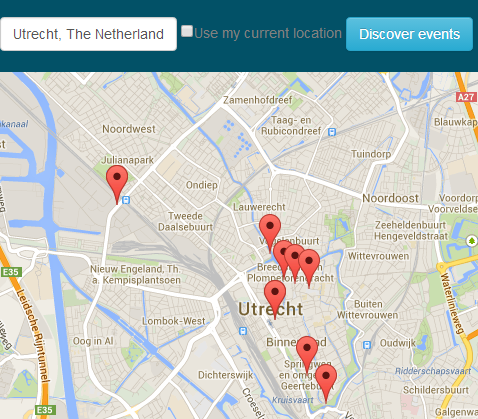
\includegraphics[scale=0.48]{images/events_utrecht.png}    
    \caption{Venues in Utrecht.}
    \label{fig:events_utrecht}
\end{figure}

\indent This kind of visualization was chosen because of its simple realization (see Section \ref{gmaps}) and of the advantages it brings: the user can easily recognize the locations closest to their own location or more accessible, and at the same time still have an overview of all the results of his search; additionally, the chosen map implementation provides a neat and simple way of displaying information about a particular location or event, as will be further explained in the following sections.

\subsection{Displaying information about events}\label{infowindow}
Once the events are correctly displayed on the map, the user will be able to access all the gathered information about them.\\
\indent The goal is to show information about the venue (See Figure \ref{fig:kerk_venue}) in which the event is held (where is it, opening hours..), accompanied by information on all the events hosted in that particular location (See Figure \ref{fig:kerk_events}), such as a general description, the starting and ending time, external links and so forth. 

\begin{figure}[h!]
  \centering
    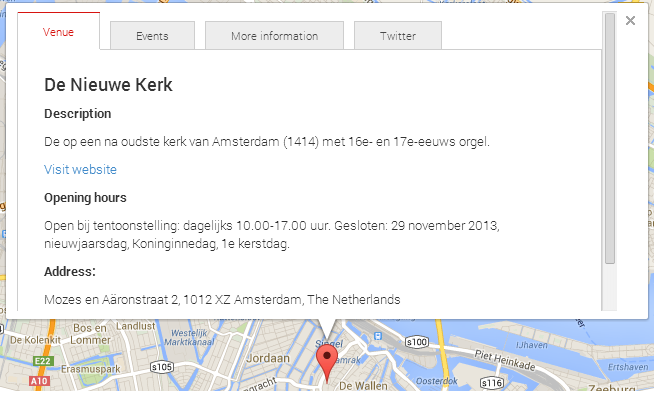
\includegraphics[scale=0.48]{images/kerk_venue.png}    
    \caption{Nieuwe Kerk in Amsterdam.}
    \label{fig:kerk_venue}
\end{figure}

\begin{figure}[h!]
  \centering
    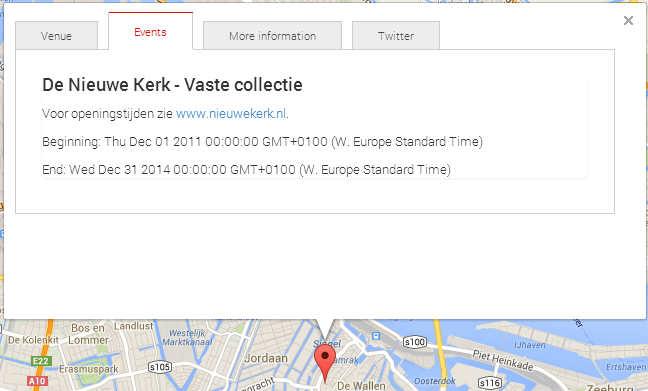
\includegraphics[scale=0.48]{images/kerk_events.png}    
    \caption{Events in the Nieuwe Kerk.}
    \label{fig:kerk_events}
\end{figure}

\indent This information will be additionally integrated with more general information about the venues e.g. description, name of the architect who designed it and its current purpose (See Figure \ref{fig:kerk_more_information}). 

\begin{figure}[h!]
  \centering
    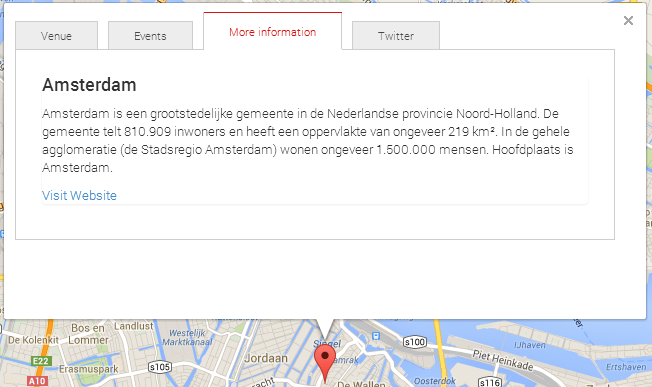
\includegraphics[scale=0.48]{images/kerk_more_information.png}    
    \caption{Additional information for the Nieuwe Kerk.}
    \label{fig:kerk_more_information}
\end{figure}

Finally, the user will be able to see all the \textit{tweets} about a particular venue done by Twitter users (See Figure \ref{fig:kerk_tweets}); this last functionality was implemented to offer a \textit{social} view of this particular web application: the user will be able to see what is the general opinion about that particular location or if other people are thinking of attending a particular event there, information that could guide his decision on which event to attend.

\begin{figure}[h!]
  \centering
    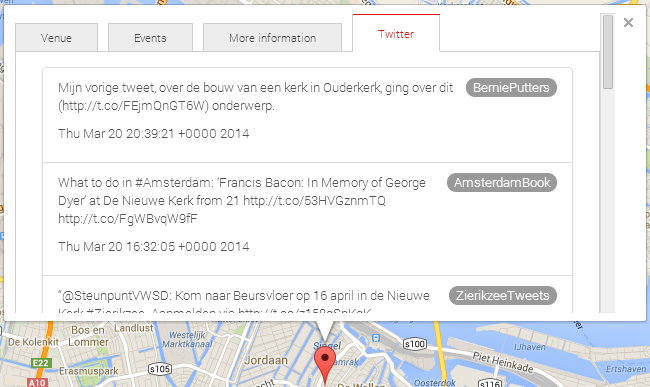
\includegraphics[scale=0.48]{images/kerk_tweets.png}    
    \caption{Twitter tweets discussing the Nieuwe Kerk.}
    \label{fig:kerk_tweets}
\end{figure}

\subsection{Statistics from the search results}

Visualization of aggregate information about the search results across more dimensions is a feature that allows the user to get a better idea on what is charachterizing the results of the entered query.

An aspect that is interesting to explore is the relationship
between a geographical location, 
venue types and the actual even genres that
carachterize venues of a certain type.

A plot with stacked bars has been added to the map in order
to provide an answer to that question.

\paragraph{Stacked visualization}
As can be seen in Figure \ref{fig:stats_stacked},
in the \emph{stacked} visualization, on the \textit{x} axis are placed all possible venue types
extracted from the results of the searched query.
The \textit{y} axis represents the amount of events in the query's results,
that belong to that specific venue type. Within the venue type's bar
are visible several stacked layers with different colors.
Each color represent a genre, which is clearly described in the legend.

In this way it's possible to see interesting correlations between venue types
and event genres.

\begin{figure}[h!]
  \centering
    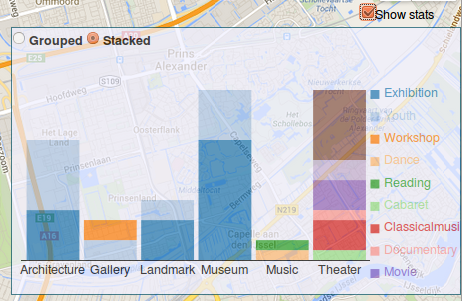
\includegraphics[scale=0.48]{images/stats_stacked.png}    
    \caption{Stacked visualization of venue type/event genre aggregates.}
    \label{fig:stats_stacked}
\end{figure}

\paragraph{Grouped visualization}
An additional \emph{grouped} visualization variant is available.
In this visualization all the layers are not anymore stacked but are placed
on the \emph{x} axis. This visualization is useful
to get a better idea of the proportions between different
\emph{venue type}/\emph{event genre} combinations.
This is clearly visible in Figure \ref{fig:stats_grouped}.

\begin{figure}[h!]
  \centering
    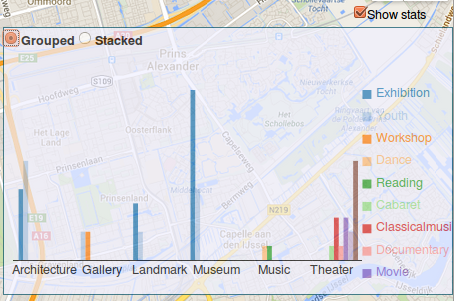
\includegraphics[scale=0.48]{images/stats_grouped.png}    
    \caption{Grouped visualization of venue type/event genre aggregates.}
    \label{fig:stats_grouped}
\end{figure}


The visualization of the stats panel can be easily toggled
via a checkbox placed on the upper right side of the map.
The visualization type can also be switched via a radio control.

The plot, produced in SVG format,
has been implemented with \emph{D3},
a flexible javascript framework that is widely
used for information visualization \cite{d3}.

\section{Datasets and services}\label{data_services}
This section discusses the datasets and services used by the application.

\subsection{ArtsHolland}
The main dataset at the base of this idea is the one provided by ArtsHolland \cite{artsholland} which contains information about events and venues in the Netherlands' biggest cities, publicly accessible cultural heritage sites, and reviews, articles and blog posts on these entities.

The data is stored in RDF format, thus obtainable with SPARQL queries, and manageable in XML or JSON. This makes it highly suited for this project and easily integrable in a web application. Through this dataset it is possible to obtain various information, such as:
\begin{itemize}

  \item information about venues (name, description, location)
  \item exact date, starting and ending time of the event
  \item the genre of the event (exhibition, etc..)
  \item the name of the event
  \item the description (both short and long)
  \item the webpage of the event
\end{itemize}

\subsection{Google Maps API} \label{gmaps}

\subsubsection{Map UI}
Google Maps Javascript API v3 \cite{gmapsv3} was used for purposes of displaying a map on the screen, alongside the necessary components that are illustrated in the map, namely the location markers and the information windows. Figure \ref{fig:google_map} exemplifies the view of the map. Section \ref{objective} presented a thorough view of the utilization of the visual map components.

\begin{figure}[h!]
  \centering
    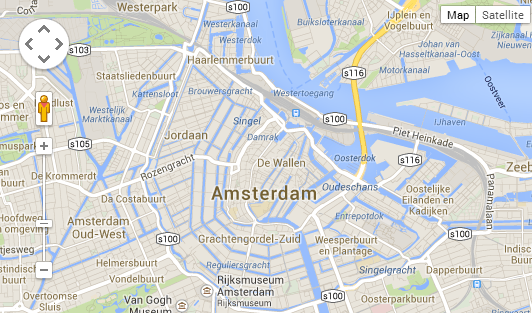
\includegraphics[scale=0.7]{images/google_map.png}    
    \caption{getaLife's map view.}
    \label{fig:google_map}
\end{figure}

\subsubsection{Places autocomplete}
The Google Maps JavaScript API v3 library for places \cite{google_places} was used to facilitate the input of a city area name in which events should be searched for (See Figure \ref{fig:location_input}). 

\begin{figure}[h!]
  \centering
    
\includegraphics[]{images/autocomplete_1.png}    
    \caption{City input box in the UI.}
    \label{fig:location_input}
\end{figure}

When the text changes withing the box, the API is configured to return city names within the Netherlands, as the ArtsHolland data only involves information regarding said country, and upon selection it will autocomplete the input term with the selected city name (See Figure \ref{fig:location_autocomplete}).

\begin{figure}[h!]
  \centering
    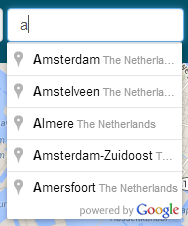
\includegraphics[]{images/autocomplete_2.png}    
    \caption{City input box autocompletion.}
    \label{fig:location_autocomplete}
\end{figure}

\subsubsection{Location detection}
The mechanism of location detection has been implemented thanks to the native geolocation functionalities in HTML5 \cite{geolocation} .\\
For this reason two factors should be held into account: 
\begin{itemize}
\item If the browser does not support HTML5, the feature will not be made available to the user;
\item For the feature to be available the user has to authorize the browser to register their actual position;
\end{itemize}
\begin{figure}[h!]
  \centering
    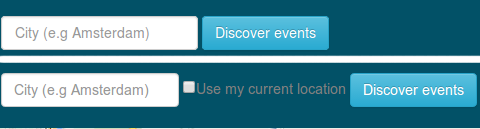
\includegraphics[height=2.5cm]{images/nogeolocation.png}    
    \caption{Search panel with and without geolocation services.}
\end{figure}
If the two previous conditions are met, the browser saves the user's current position, that will be converted by the web application into coordinates in a format compatible with Google APIs for further use (see Section \ref{geocoding}).
\subsubsection{Geocoding and reverse geocoding} \label{geocoding}
The Google Maps JavaScript API v3 Geocoding Service \cite{google_geocoding} is used in two places within the application: when selecting a location for the search parameters and when displaying the address of a venue.

When selecting a location for the search parameters from the autocomplete box, the geocoding service is queried with this location name and the geocoordinate bounds for this location are extracted, which in turn are used as part of the query to the RDF store, ensuring that the venues to be retrieved are inside this bounding box.

For example, if the selected city is \emph{Amsterdam, The Netherlands} the bounding box can be determined from the data retrieved from Google (See Figure \ref{fig:geocoding_amsterdam}). The relevant geocoordinates, in this particular case, are: 

\begin{itemize}
  \item \textbf{North:} 52.4311573
  \item \textbf{South:} 52.3182742
  \item \textbf{West:} 4.728855800000019
  \item \textbf{East:} 5.068377499999997
\end{itemize}

\begin{figure}[h!]
  \centering
    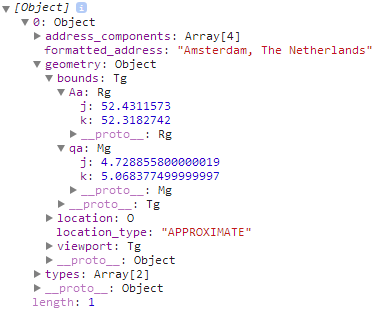
\includegraphics[]{images/geocode_amsterdam.png}    
    \caption{Geocoding information for Amsterdam.}
    \label{fig:geocoding_amsterdam}
\end{figure}

The reverse geocoding service from Google \cite{reverse_geocoding} is used when retrieving the venues information from the RDF store. Each venue has a latitude and longitude that is used to display a marker on the map. However, far more interesting for the user, would be to be able to know the location's address. To achieve just this, Google's service is queried with the geocoordinates on the venue and from the response  the address is taken out and then used in the venue information window .

Figure \ref{fig:reverse_geo_response} shows the JSON response of reverse geocoding the location of \emph{Van Eesterenmuseum} showcasing the formatted address. Figure \ref{fig:reverse_geocoding_address} displays the venue information window containing the more user-friendly address.

\begin{figure}[h!]
  \centering
    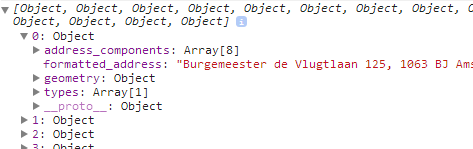
\includegraphics[]{images/geocode_find_address_response.png}    
    \caption{Reverse geocoding JSON response for \emph{Van Eesterenmuseum}.}
    \label{fig:reverse_geo_response}
\end{figure}

\begin{figure}[h!]
  \centering
    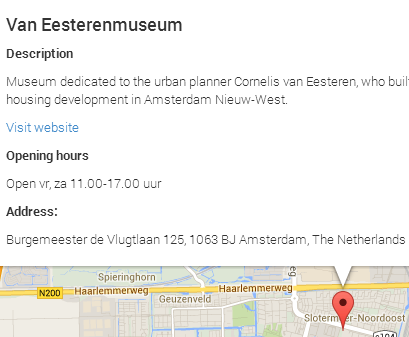
\includegraphics[]{images/geocode_find_address.png}    
    \caption{Displaying venue address.}
    \label{fig:reverse_geocoding_address}
\end{figure}


\subsection{Foursquare}\label{foursquare}
Foursquare's Search Venues API \cite{foursquare_api} was used for purposes of performing inferencing in the knowledge base (see Section \ref{inferencing}). Missing information (i.e. the geolocation and homepage) about some venues in the ArtsHolland data was extracted from Foursquare to make the stored information more complete.

As an example, the following block of code represents data in Turtle format about the \emph{Mirliton theater}:

\indent
\begin{verbatim}
fs:4cb441d775ebb60cc2eae0ad a fs:Venue;
      fs:title "Mirliton theater"@nl;
      geo:lat "52.0905950494175"^^xsd:float;
      geo:long "5.115401744842529"^^xsd:float;
      foaf:homepage <http://www.mirliton.nl>.
\end{verbatim}

\subsection{Twitter}
Twitter's search API \cite{twitter_api} is used to retrieve a mix of both recent and popular tweets about the venue being currently displayed (see Figure \ref{fig:kerk_tweets} in Section \ref{infowindow}). When the user clicks on a venue marker on the map, the venue name and it's geocoordinates are extracted and used to query for tweets discussing the venue, giving preference to tweets created near the venue's location. Figure \ref{fig:twitter_response} shows an example response from the Twitter Search API.

Each tweet's id, text, user and date are extracted. The text, user and date are displayed to the user, and the id is utilized to construct a hyperlink to the original tweet.

\begin{figure}[h!]
  \centering
    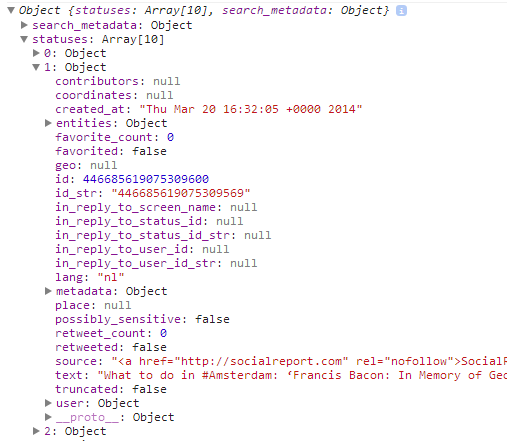
\includegraphics[]{images/twitter_response.png}    
    \caption{Twitter's response for a query about \emph{"De Nieuwe Kerk"}.}
    \label{fig:twitter_response}
\end{figure}

\subsection{DBPedia}
To further integrate the data obtained up until this point, the application exploits the great variety of information available on DBPedia.
Every location hosting events located on the map contains, in the information window that opens on click, a section reserved specifically for this kind of data: when possible, further information about the location were obtained (such as name of the architect who designed it, its current purpose and so on); whenever this information was not available, generic information about the citythe location is situated in is shown.

\begin{figure}[h!]
  \centering
    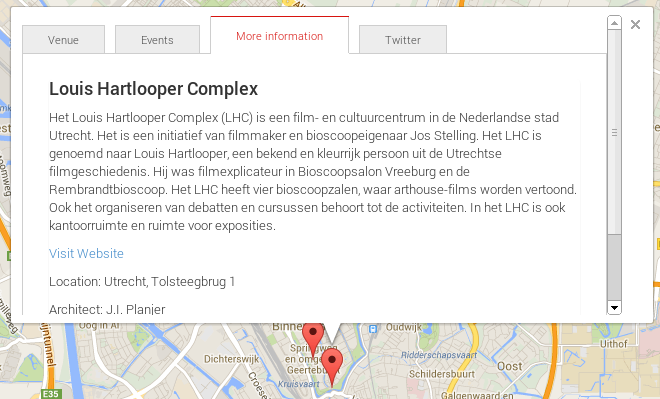
\includegraphics[scale=0.5]{images/infoDBP1.png}    
    \caption{Example of venue-related information from DBPedia.}
\end{figure}

\begin{figure}[h!]
  \centering
    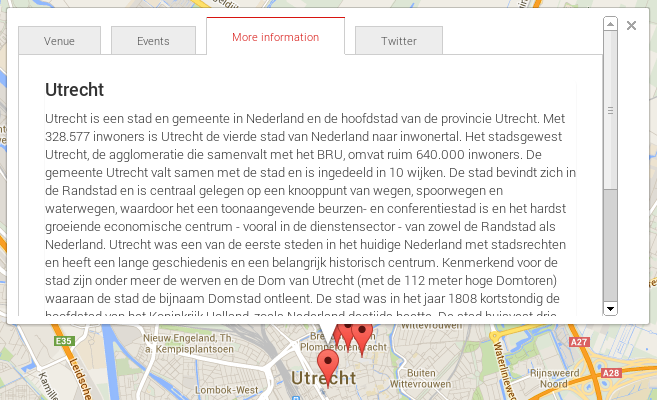
\includegraphics[scale=0.5]{images/inforDBP2.png}    
    \caption{Example of city-related information from DBPedia.}
\end{figure}

To be able to find a greater amount of information about Netherland-specific location, \textit{nl.dbpedia.org} was used instead of the generic \textit{dbpedia.org}.

\section{Inferencing}\label{inferencing}
As stated in Section \ref{foursquare}, some of the venues in the ArtsHolland data was missing some information, which was crucial to the web-application. In concrete, some venues were missing the geocoordinates, and without them the venue cannot be displayed on the map, and by transition neither can the events associated to it. Figure \ref{fig:ah_miss_data} shows an excerpt of venue data. As it can be seen, a venue like the \emph{Mirliton theater} is missing the latitude and longitude values.

\begin{figure}[h!]
  \centering
    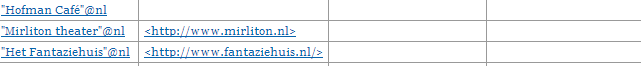
\includegraphics[scale=0.6]{images/venues_missing_data.png}    
    \caption{Venues with missing data.}
    \label{fig:ah_miss_data}
\end{figure}

The following block of code represents data in Turtle format about the \emph{Mirliton theater}, data that was extracted from Foursquare:

\begin{center}
\begin{verbatim}
fs:4cb441d775ebb60cc2eae0ad a fs:Venue;
      fs:title "Mirliton theater"@nl;
      geo:lat "52.0905950494175"^^xsd:float;
      geo:long "5.115401744842529"^^xsd:float;
      foaf:homepage <http://www.mirliton.nl>.
\end{verbatim}
\end{center}

These triple statetements in combination with an inferencing rule that determines that venues with the same homepage are in fact the same was then used as means to augment the AH data. The rule in question is shown in the following block of Turtle code:

\begin{center}
\begin{verbatim}
foaf:homepage rdf:type owl:InverseFunctionalProperty .
\end{verbatim}
\end{center}

Once the rule and the data from Foursquare are in the knowledge store, a second look at the data reveals more completeness, as seen in Figure \ref{fig:ah_more_data}

\begin{figure}[h!]
  \centering
    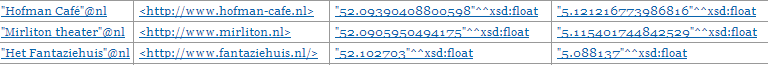
\includegraphics[scale=0.6]{images/venues_complete_data.png}    
    \caption{Venues with complete data.}
    \label{fig:ah_more_data}
\end{figure}

\section{Implementation considerations}\label{considerations}

\subsection{Application Architecture}

A three-tier application architecture model was following for the implementation of the web application. The general model is depicted in Figure \ref{fig:architecture}.

\begin{figure}[h!]
  \centering
    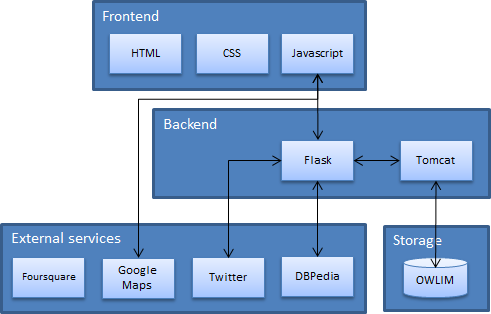
\includegraphics[scale=1.0]{images/architecture.png}    
    \caption{Architecture of getaLife.}
    \label{fig:architecture}
\end{figure}

The frontend was built using HTML, CSS and Javascript. The Javascript code queries \emph{RESTfully} the Flask server in the backend, which is in charge of retrieving data from the OWLIM knowledge base, DBPedia and Twitter. The Javascript also communicates with the Google Maps Javascript API for geolocation related activities and map visualization. It's worth mentioning that OWLIM also allowed for the capability of providing our very own sparql endpoint.

The Foursquare external service is disconnected from everything due to some constraints in the retrieval of the data. See Section \ref{manual_foursquare} for an explanation.

Some of the different software used by application are:

\begin{itemize}
  \item Google Maps Javascript API v3 \cite{gmapsv3}
  \item JQuery 1.11.0 \cite{jquery}
  \item Bootstrap 3.1.1 \cite{bootstrap}
  \item Bootstrap Dialog \cite{bootstrap-dialog}
  \item Bootstrap Dropdown Checkbox \cite{bootstrap-dropdown-checkbox}
  \item Bootstrap Datepicker \cite{bootstrap-datepicker}
  \item Ion Tabs 1.0.2 \cite{ion-tabs}
  \item Python 2.7 \cite{python}
  \item Flask 0.10 \cite{flask}
  \item OWLIM lite 5.4.6486 \cite{owlim}
  \item Apache Tomcat 7.0.52 \cite{tomcat}
\end{itemize}

\subsection{Getting data from ArtsHolland}
Extracting data from the ArtsHolland Sparql endpoint \cite{artsholland_sparql} was quite problematic. The endpoint was quite unstable and was often down when data was needed for retrieval, in addition to frequently truncating the response to a query. In the end, queries with limits and offset were used to dump the data for Venues, Events, Production and Genres, but only for those entities that relate to events that are active beyond \emph{2014-03-12}, anything before that (i.e. things that are not longer relevant), were of no interest. 

Even though the data was dumped by querying the AH sparql endpoint, running the same query on the AH website itself yieled far more results. We are still baffled at this, and could not figure out why the reason for this was. Regardless, the (what seems limited) data that was managed to be dumped servers the purpose of being illustrative for the application's proof of concept.

The dumped data was loaded in a local knowledgebase to avoid all the mentioned  problems, and to ease the activities relating to inferencing (see Section \ref{inferencing}), as the data was in need of being augmented or curated.

\subsection{Getting data from DBPedia}
In obtaining data from DBPedia we encountered a quite relevant obstacle: the names of the venues as presented in ArtsHolland did not correspond to the ones offered in the DBPedia dataset. For example, the venue presented as "De Nieuwe Kerk" from ArtsHolland, is found on DBPedia as "Nieuwe Kerk"; as such, when querying the dataset for venues, this venue is simply catalogued as \textit{not found} and ignored. \\
\indent In a future, more advanced implementation of this web application it would be nice to be able to automate the search for partial names, using SPARQL filtering function and regulare expression for string matching.

\subsection{Getting data from Foursquare}\label{manual_foursquare}
The data extracted from Foursquare (see Section \ref{foursquare}) was retrieved in a manual fashion, as the names for the venues in the ArtsHolland data did not necessarily match the name that the venue had in Foursquare, making it really difficult to automate the process, as doing so would likely leave the data with some strange results. To circumvent this, the queries to Foursquare and the subsequent data extraction was done manually and with much care to find the appropriate venues.

\section{Future work}\label{future_work}
Before considering expanding the web application, it must be pointed out that the ArtsHolland dataset is quite outdated and not so easily manageable as initially thought. A nice objective for the future should be to find a way to keep the ArtsHolland dataset continuously updated, because as it has been shown with this project, it can be source of inspiration for useful applications.\\
\indent Nonetheless, in the following paragraphs are presented some nice idea to expand the \textit{getaLife} application.

\paragraph{Adding transportations information:}
once the current location of the user and the selected events are known, it would be quite easy to integrate a functionality that allows the user to choose a preferred transoportation mean, and show him the correct route to arrive to their destination. Such information is already partially available in ArtsHolland (e.g. Tram lines that connect you to the chosen event), so that could be a good point to start developing this new feature.

\paragraph{Exporting the events into calendars:}
an interesting possible improvement could be the exporting of the events in a standard format (for example \emph{iCal}) or to specific applications, such as \emph{Google Calendar}. This extraction could be done automatically, as a subscription service. This way a user could be
constantly updated about his preferred events by just checking his calendar.

\paragraph{Studying trends:}
it can be useful to see, as time goes by, how certain event typologies become more or less popular than others.
This kind of knowledge can of course be used for marketing purposes, but can also be helpful for policy making. The use of the map as a central element in the exploration of data, combined with graphic representation of the events' data in their several dimensions, can for example facilitate the observation that in a certain part of a city there is lack of cultural offer. Counteracting this tendence may improve the chances of establishing a sense of community in socially disgregated suburbs.


\section{Conclusions}\label{conclusions}
Despite the fact that the application fulfills all the initial requirements, as we pointed out in the previous section there is always room for improvement. Even though Semantic Web proved itself to be a great tool with which to handle data and knowledge, many are the problems that a developer can face, first and most important of all the lack of data and the different representation for the same entities chosen by different centralized datasets, such as DBPedia, ArtsHolland or Foursquare. \\
\indent Another obstacle can be found in the fact that not all data centers use rdf notation to represent their own data, so a lot of different representations are available on the entirety of the World Wide Web. \\
\indent Regardless of these difficulties, using Open Data allows for great accessibility of data, increasing enormously the potential of web applications, and guarantees for data reusability and recombination to obtain continuously new information. In conclusion, working with Semantic Web was certainly a way to understand why such a notation important and should be exploited to its full potential.
\newline \\
Note: a link to a functioning version of the web aplication can be found at \url{http://54.186.171.129:5000/}

\section*{References}
\addcontentsline{toc}{section}{References}

\begingroup
\renewcommand{\section}[2]{}%

\begin{thebibliography}{99}

\bibitem{google_places}
	Google Maps JavaScript API v3,
    \emph{Places Library}
    \url{https://developers.google.com/maps/documentation/javascript/places},
    Visited: 18-03-2014
    
\bibitem{google_geocoding}
	Google Maps JavaScript API v3,
    \emph{Geocoding Service}
    \url{https://developers.google.com/maps/documentation/javascript/geocoding},
    Visited: 18-03-2014

\bibitem{reverse_geocoding}
	Google Maps JavaScript API v3,
    \emph{Reverse Geocoding}
    \url{https://developers.google.com/maps/documentation/javascript/geocoding#ReverseGeocoding},
    Visited: 18-03-2014

\bibitem{geolocation}
	W3Schools, 
	\emph{HTML5 Geolocation},
    \url{http://www.w3schools.com/html/html5_geolocation.asp}, Visited: 20-03-2014
    
\bibitem{twitter_api}
	Twitter,
    \emph{Search API}
    \url{https://dev.twitter.com/docs/using-search},
    Visited: 21-03-2014
    
\bibitem{foursquare_api}
	Foursquare,
    \emph{Search Venues}
    \url{https://developer.foursquare.com/docs/venues/search},
    Visited: 21-03-2014
    
\bibitem{bootstrap-dialog}
	Bootstrap Dialog,
    \url{http://nakupanda.github.io/bootstrap3-dialog/},
    Visited: 21-03-2014
    
\bibitem{bootstrap-datepicker}
	Datepicker for Bootstrap,
    \url{http://www.eyecon.ro/bootstrap-datepicker/},
    Visited: 21-03-2014
    
\bibitem{bootstrap}
	Bootstrap,
    \url{http://getbootstrap.com/},
    Visited: 21-03-2014
    
\bibitem{bootstrap-dropdown-checkbox}
	Bootstrap Dropdown Checkbox,
    \url{https://github.com/Acquisio/bootstrap-dropdown-checkbox},
    Visited: 21-03-2014
    
\bibitem{ion-tabs}
	Ion.Tabs,
    \url{https://github.com/IonDen/ion.tabs},
    Visited: 21-03-2014
    
\bibitem{jquery}
	jQuery,
    \url{http://jquery.com/},
    Visited: 21-03-2014

\bibitem{d3}
	D3,
    \url{http://d3js.org/},
    Visited: 21-03-2014

\bibitem{python}
	Python 2.7,
    \url{https://www.python.org/download/releases/2.7/},
    Visited: 21-03-2014
    
\bibitem{flask}
	Flask 0.10,
    \url{http://flask.pocoo.org/},
    Visited: 21-03-2014
   
\bibitem{owlim}
	OWLIM lite 5.4.6486,
    \url{https://www.ontotext.com/owlim},
    Visited: 21-03-2014 

\bibitem{tomcat}
	Apache Tomcat 7.0.52,
    \url{http://tomcat.apache.org/},
    Visited: 21-03-2014 

\bibitem{gmapsv3}
	Google Maps Javascript API v3,
    \url{https://developers.google.com/maps/documentation/javascript/},
    Visited: 21-03-2014

\bibitem{artsholland}
	Arts Holland Platform,
    \url{http://dev.artsholland.com/},
    Visited: 21-03-2014
    
\bibitem{artsholland_sparql}
	Arts Holland Sparql Endpoint,
    \url{http://api.artsholland.com/sparql},
    Visited: 21-03-2014
    
\end{thebibliography}



\endgroup


\end{document}
